\documentclass[10pt]{extarticle}

\usepackage[margin=0.72in]{geometry}
\usepackage{amsmath,amssymb,amsthm,mathtools}
\usepackage{booktabs}
\usepackage{array}
\newcolumntype{L}[1]{>{\raggedright\arraybackslash}p{#1}}
\usepackage{enumitem}
\usepackage{hyperref}
\usepackage{microtype}
\usepackage{tikz}
\usetikzlibrary{arrows.meta,positioning,calc,fit}

\hypersetup{
  colorlinks=true,
  linkcolor=blue,
  urlcolor=blue,
  pdftitle={ZenoDEX Whitepaper: Full-System Architecture, Public Assurance Boundary, and Proof Agenda},
  pdfauthor={Dana Edwards}
}
\setlist[enumerate]{nosep,leftmargin=5mm}
\setlength{\textfloatsep}{8pt plus 1pt minus 2pt}
\setlength{\floatsep}{8pt plus 1pt minus 2pt}
\setlength{\intextsep}{8pt plus 1pt minus 2pt}
\setlength{\abovedisplayskip}{7pt}
\setlength{\belowdisplayskip}{7pt}
\setlength{\abovecaptionskip}{4pt}
\setlength{\belowcaptionskip}{0pt}

\newcommand{\tuple}[1]{\langle #1 \rangle}
\newcommand{\Exec}{\mathsf{Exec}}
\newcommand{\Guards}{\mathsf{Guards}}
\newcommand{\Cert}{\mathsf{Cert}}
\newcommand{\Risk}{\mathsf{Risk}}
\newcommand{\Runtime}{\mathsf{Runtime}}
\newcommand{\Assure}{\mathsf{Assure}}
\newcommand{\Key}{\mathsf{Key}}
\newcommand{\Winner}{\mathsf{Winner}}
\newcommand{\argmin}{\operatorname*{arg\,min}}
\newcommand{\code}[1]{\path{#1}}

\newtheorem{claim}{Claim}

\title{ZenoDEX Whitepaper: Full-System Architecture, Public Assurance Boundary, and Proof Agenda}
\author{Dana Edwards}
\date{April 2026}

\begin{document}
\maketitle

\begin{abstract}
ZenoDEX is intended to be a proof-carrying exchange architecture rather than a
collection of isolated trading scripts. The intended full system spans integer
spot execution kernels, theorem-backed canonical winner relations, fail-closed
Tau and ESSO guard layers, settlement and oracle certificate planes, bounded
stablecoin and perpetual-risk slices, narrow replayable runtime adapters, and a
public assurance surface that can be rebuilt from a clean checkout. This
whitepaper describes that full target architecture, states the current public
assurance boundary, and names the remaining proof obligations required to close
the gap between the present public claim and the end-state system.
\end{abstract}

\paragraph{Contributions.}
This whitepaper contributes:
\begin{enumerate}
  \item a decomposition of ZenoDEX into execution, guard, certificate, risk,
  runtime, and assurance planes;
  \item an explicit evidence discipline that separates proved,
  contract-backed, implemented, replay-backed, and still-open claims;
  \item a public-safe guarantee-and-assumption matrix for the major protocol
  surfaces;
  \item a whole-system proof agenda that states what the architecture still
  needs beyond the current RC1 public surface.
\end{enumerate}

\section{System thesis}
The intended full architecture is
\[
\mathsf{ZenoDEX}
:= \Exec \wedge \Guards \wedge \Cert \wedge \mathsf{Control}
\wedge \mathsf{Oracle} \wedge \mathsf{zUSD} \wedge \mathsf{Perps}
\wedge \Runtime \wedge \Assure.
\]
Standard reading: the system is the conjunction of value-moving execution,
fail-closed guards, certificate-carrying settlement and oracle lanes, monetary
and derivatives risk layers, narrow runtime adapters, and replayable assurance
artifacts.
Practical consequence: the whole system cannot be judged only by the spot math
or only by the API shell. The architecture claim is inherently cross-layer.

The corresponding public discipline is
\[
\mathsf{PublicClaim} \subset \mathsf{EvidenceFrontier} \subset \mathsf{FullTargetArchitecture}.
\]
Standard reading: the public release claim is narrower than the strongest
current evidence frontier, and the evidence frontier is narrower than the full
intended architecture.
Practical consequence: this paper can describe the whole target system in
detail without pretending that every described surface is already proved or
release-backed.

\begin{figure}[t]
\centering
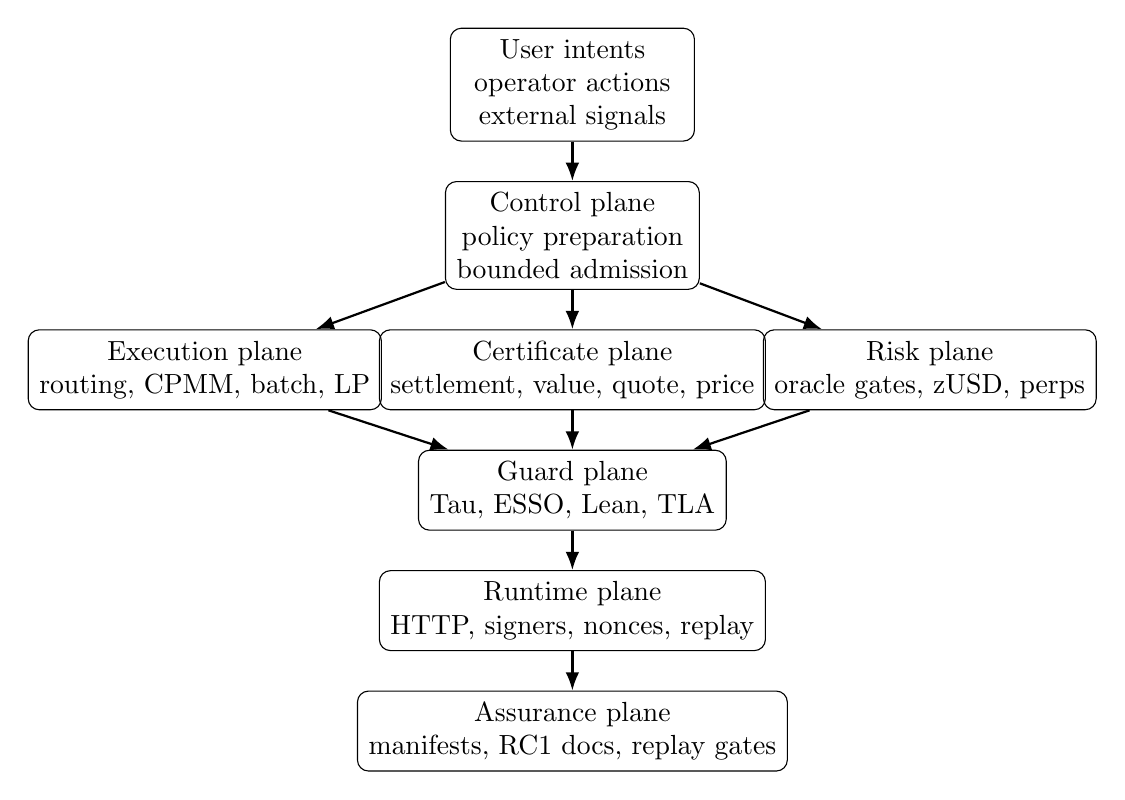
\begin{tikzpicture}[
  node distance=5mm and 8mm,
  box/.style={draw, rounded corners, align=center, inner sep=4pt, minimum width=31mm},
  arr/.style={-Latex, thick}
]
\node[box] (intent) {User intents\\operator actions\\external signals};
\node[box, below=of intent] (control) {Control plane\\policy preparation\\bounded admission};
\node[box, below left=of control] (exec) {Execution plane\\routing, CPMM, batch, LP};
\node[box, below=of control] (settle) {Certificate plane\\settlement, value, quote, price};
\node[box, below right=of control] (risk) {Risk plane\\oracle gates, zUSD, perps};
\node[box, below=of settle] (guards) {Guard plane\\Tau, ESSO, Lean, TLA};
\node[box, below=of guards] (runtime) {Runtime plane\\HTTP, signers, nonces, replay};
\node[box, below=of runtime] (assure) {Assurance plane\\manifests, RC1 docs, replay gates};
\draw[arr] (intent) -- (control);
\draw[arr] (control) -- (exec);
\draw[arr] (control) -- (settle);
\draw[arr] (control) -- (risk);
\draw[arr] (exec) -- (guards);
\draw[arr] (settle) -- (guards);
\draw[arr] (risk) -- (guards);
\draw[arr] (guards) -- (runtime);
\draw[arr] (runtime) -- (assure);
\end{tikzpicture}
\caption{The intended full ZenoDEX stack. Execution authority flows only through fail-closed guards and narrow runtime adapters.}
\label{fig:stack}
\end{figure}

\section{Evidence discipline}
The governing evidence order is
\[
\mathtt{proved} > \mathtt{contract} > \mathtt{implemented} > \mathtt{replay\_backed} > \mathtt{hypothesis}.
\]
Standard reading: a claim may only be stated at the strongest replayable
support the repository actually carries.
Practical consequence: this paper treats theorem-bearing spot slices,
manifest-backed contract surfaces, and replayable release evidence differently
rather than collapsing them into one generic ``verified'' label.

The paper uses four recurring claim shapes:
\[
C \neq \varnothing \to \exists !\, w \in C \text{ such that } \forall c \in C,\; \Key(w) \le \Key(c),
\]
\[
\mathsf{CertificateOK} \to \mathsf{CanonicalPayload} \wedge \mathsf{ReplayCheckable},
\]
\[
\mathsf{RiskTransitionAllowed} \to \mathsf{OracleAligned} \wedge \mathsf{BoundedMove} \wedge \mathsf{LocalInvariantOK},
\]
\[
\mathsf{ReleaseClaimOK} := \mathsf{CleanTree} \wedge \mathsf{ScopeFrozen} \wedge \mathsf{ReplayGreen} \wedge \mathsf{ExclusionsHonest}.
\]
Standard reading: canonical winner, proof-carrying packets, bounded risk
transitions, and replay-backed release posture are the four main logical forms
used across the system.
Practical consequence: the assurance story is compositional. The paper does not
need one single monolithic theorem to still be technically coherent.

\section{Control plane}
The control plane is the whole-system layer that turns raw operator or user
requests into admissible execution candidates. It is narrower than the advisory
layer, but broader than the execution core.
Its intended law is
\[
\mathsf{AdmittedIntent}
:= \mathsf{NormalFormOK}
\wedge \mathsf{SignatureOrWitnessOK}
\wedge \mathsf{NonceOK}
\wedge \mathsf{KindSupported}
\wedge \mathsf{BoundaryContractOK}.
\]
Standard reading: before the execution plane is even allowed to compare route
or settlement candidates, ingress must already be normalized, authenticated,
nonce-consistent, supported by the current release contract, and within the
documented runtime boundary.
Practical consequence: the system should be reviewed as
\emph{admit then optimize}, not as \emph{optimize then try to reject dangerous
payloads later}.

The public-safe control responsibilities are:
\begin{enumerate}
  \item normalize user intents into canonical payloads;
  \item bind signatures, witness packets, and nonces to those payloads;
  \item reject unsupported action families or malformed envelope shapes;
  \item carry forward only the bounded action language that the release surface
  actually supports.
\end{enumerate}

This layer is therefore the bridge between the runtime plane and the execution
plane. A DEX paper that omits it would miss how replay safety and canonicality
are coupled in practice.

\section{Execution plane}
\subsection{Spot routing and canonicality}
The public execution core is built around explicit candidate families and total
keys. The intended winner semantics is
\[
\Winner(C) := \argmin_{c \in C} \Key(c).
\]
Standard reading: on a bounded emitted candidate family, the chosen route or
batch outcome is the unique minimum under an explicit total key.
Practical consequence: deterministic replay is upgraded from ``same loop order''
to a semantic canonicality claim.

The strongest current public posture is theorem-bearing on bounded candidate
families rather than universal over all conceivable route generators. The key
public references are the Lean winner theorems and the release-facing exact-in,
exact-out, and batch certificate surfaces described in:
\begin{itemize}
  \item \code{lean-mathlib/Proofs/BatchAuctionCanonical.lean}
  \item \code{lean-mathlib/Proofs/ZenoDEXExactInTrueKeyWinner.lean}
  \item \code{docs/RC1_VERIFIED_SURFACE_MATRIX.md}
\end{itemize}

\subsection{CPMM and accounting}
The spot core also relies on explicit integer arithmetic contracts:
\[
\mathsf{amount\_out} < \mathsf{reserve\_out},
\qquad
K_{after} \ge K_{before}
\text{ in the zero-fee integer reference model},
\]
with fee-side accounting shaped by
\[
\mathsf{fee\_conserved} \wedge \mathsf{dust\_carry\_bounded}.
\]
Standard reading: reserve-bounded swap execution and exact fee accounting are
first-class contracts, not informal expectations.
Practical consequence: any whole-system settlement or runtime claim inherits
these accounting constraints as preconditions.

\subsection{Batch execution and LP semantics}
Batch execution adds two additional structures:
\[
\mathsf{ValidOutcome}(B) \to \mathsf{CanonicalBatchWinner}(B) \wedge \mathsf{SettlementMeaningful}(B),
\]
\[
\mathsf{LPRoundTrip} \to \mathsf{NoImmediateValueCreation}.
\]
Standard reading: valid batch outcomes must produce canonical winners and
meaningful settlements, and LP mint/burn semantics should reject immediate
value-creation folklore.
Practical consequence: the paper treats batch execution and LP mechanics as
part of the same execution plane, not as detached utilities.

\section{Guard plane}
The guard plane is intentionally redundant. ZenoDEX relies on several distinct
kinds of guard rails:
\begin{enumerate}
  \item Tau specs for fail-closed stream and policy boundaries;
  \item ESSO kernels for bounded transition-system verification and solver
  cross-checking;
  \item Lean proofs for canonicality, accounting, and algebraic helper laws;
  \item bounded TLA/TLC shadow models for release-facing temporal claims.
\end{enumerate}

The role of this plane is expressed by
\[
\mathsf{ExecutionAuthority} \to \mathsf{GuardedByTauOrKernelOrProofBackedShell}.
\]
Standard reading: authority-bearing transitions should only occur when they are
filtered by an explicit public guard surface.
Practical consequence: the architecture is not satisfied by tests alone; it
requires a layered acceptance posture.

\section{Certificate plane}
The certificate plane is where the architecture becomes explicitly
proof-carrying rather than merely deterministic.

\subsection{Quote and settlement certificates}
The guiding law is
\[
\mathsf{SettlementOK}
\to \mathsf{CanonicalDeltaTable}
\wedge \mathsf{QuoteOrKernelWitnessBound}
\wedge \mathsf{ReplayVerifiable}.
\]
Standard reading: accepted settlement must carry canonical deltas, bind fills to
quote or kernel witnesses, and remain replay-checkable.
Practical consequence: settlement is a certified boundary object, not just a
serialized runtime decision.

This certificate family includes:
\begin{itemize}
  \item quote receipts and their verification surfaces;
  \item settlement strong certificates;
  \item end-to-end settlement certificate packets;
  \item value packets and endogenous LP value packets;
  \item price provenance and signed attestation packets.
\end{itemize}

\subsection{Composition discipline}
The composition law across packet and kernel boundaries is
\[
\mathsf{SharedFactInA} = \mathsf{MirrorOfFactInB}
\quad \text{must be preserved after every relevant transition.}
\]
Standard reading: any fact shared across modules must be mirrored and kept
synchronized inductively, not repaired later by convention.
Practical consequence: composition is part of the proof surface, not only part
of the engineering style guide.

\section{Oracle and price plane}
ZenoDEX treats price and oracle material as a first-class plane rather than as
ambient input. The intended safety contract is
\[
\mathsf{PriceInputAccepted}
\to \mathsf{FreshnessBound}
\wedge \mathsf{SourceBound}
\wedge \mathsf{PendingStateConsistent}
\wedge \mathsf{ProvenancePacketCoherent}.
\]
Standard reading: accepted price material must satisfy freshness limits, source
restrictions, pending-vs-active state consistency, and provenance coherence.
Practical consequence: any stablecoin, settlement, or perps claim inherits a
price-admission contract rather than merely trusting a floating external
number.

This plane is wider than one oracle adapter. It includes:
\begin{itemize}
  \item price provenance packets and optional attestation surfaces;
  \item active-vs-pending oracle transition discipline;
  \item quote freshness and settlement snapshot alignment;
  \item cross-module oracle alignment assumptions used by zUSD and perps.
\end{itemize}

The key architecture point is that oracle posture is not just a risk-layer
detail. It constrains admission, settlement, and liquidation semantics across
the system.

\section{Runtime plane}
The public runtime surface is deliberately narrower than the repository.
The supported ingress contract is documented rather than inferred.
Its public-safe reading is
\[
\mathsf{SupportedHTTP} \subset \mathsf{AllRuntimeEndpoints}.
\]
Standard reading: the supported public runtime path is a bounded subset of the
possible API and integration surfaces.
Practical consequence: a whole-system paper should describe the full runtime
stack while still naming the narrower release-backed boundary.

The runtime plane itself includes:
\begin{itemize}
  \item supported HTTP handlers for quote and settlement packet work;
  \item signer, nonce, and receipt binding surfaces;
  \item snapshot recovery and deterministic serialization boundaries;
  \item Tau testnet adapters and plugin shells;
  \item replay and gate wrappers used to rebuild the public assurance surface.
\end{itemize}

A representative runtime invariant is
\[
\mathsf{SignedOrWitnessedIngress} \to \mathsf{NonceConsistent} \wedge \mathsf{ReceiptConsistent} \wedge \mathsf{CanonicalPayloadConsistent}.
\]
Standard reading: admitted runtime ingress must bind signer, nonce, receipt,
and canonical payload views consistently.
Practical consequence: replay safety depends as much on ingress discipline as on
execution math.

The replay-critical runtime subfamilies are:
\begin{enumerate}
  \item request-envelope validation and intent authentication;
  \item quote-receipt transport and stale-receipt rejection;
  \item nonce state transitions, replay prevention, and sequence monotonicity;
  \item snapshot encode/decode and restart recovery.
\end{enumerate}
These are the surfaces where a public release can look ``mathematically safe''
on paper while still failing operationally if the ingress shells drift.

\section{Risk and monetary planes}
\subsection{zUSD}
The public zUSD posture is narrower than a full stablecoin completeness proof,
but the intended invariant shape is already explicit:
\[
\mathsf{zUSDAdmissible} \to \mathsf{DebtConservation} \wedge \mathsf{CollateralConservation}.
\]
The oracle safety side is shaped by
\[
\mathsf{price\_pending} \neq \mathsf{price} \to \mathsf{RiskyTransitionsBlocked}.
\]
Standard reading: zUSD actions are only admissible when both balance laws hold,
and stale or pending oracle posture blocks risky transitions.
Practical consequence: debt-only reasoning is not an adequate public safety
story for the monetary layer.

The intended zUSD substructure is:
\begin{itemize}
  \item mint, repay, withdraw-collateral, liquidation, and risky-ops gates;
  \item oracle-commit and multi-oracle alignment contracts;
  \item debt and collateral conservation helper theorems;
  \item runtime token and wallet boundaries that must preserve the same
  monetary semantics.
\end{itemize}
Standard reading: zUSD is not one theorem or one Python module. It is a family
of balance laws, admission contracts, and oracle-state gates that must remain
consistent across kernel, runtime, and wallet-adjacent surfaces.
Practical consequence: a full-system paper has to describe the stablecoin plane
as a composition problem, not only as a mint/redeem formula.

\subsection{Perps}
The intended perpetual-risk law is bounded rather than universal:
\[
\mathsf{PerpTransitionAllowed}
\to \mathsf{FreshOracleWindow}
\wedge \mathsf{BoundedMoveGate}
\wedge \mathsf{FundingOrSettlementWitnessOK}.
\]
Standard reading: the perps layer relies on explicit oracle freshness, bounded
moves, and witness-backed settlement or funding lanes.
Practical consequence: the paper can cover the perps plane in detail without
claiming that every derivatives surface is already release-authoritative.

The intended perps plane includes:
\begin{itemize}
  \item funding epoch and settlement witness lanes;
  \item bounded-move and insurance-envelope guards;
  \item liquidation containment contracts;
  \item public API and settlement shells that mirror the same bounded semantics.
\end{itemize}
Standard reading: the perps plane is a bounded risk machine, not a generic
unconstrained derivatives engine.
Practical consequence: the correct public claim is a bounded envelope posture,
not ``all derivatives semantics are fully solved''.

\section{Control and advisory surfaces}
The full intended system contains non-authoritative control and preparation
surfaces: policy compilation, operator configuration, safety review, and
bounded recommendation layers.
The public safety law is
\[
\mathsf{AdvisoryPlane} \to \mathsf{NonAuthoritative},
\qquad
\neg(\mathsf{AdvisoryPlane} \to \mathsf{BalanceMovingAuthority}).
\]
Standard reading: planning or ranking surfaces may influence what operators look
at, but they do not gain direct value-moving authority.
Practical consequence: the whole-system paper includes these layers because they
shape the intended architecture, but they remain outside the core public RC1
execution claim.

\section{Assurance plane}
The assurance plane is the layer that turns the architecture into a replayable
public claim. Its operating law is
\[
\mathsf{PublishedClaimOK}
\to \mathsf{ManifestPinned}
\wedge \mathsf{ReplaySurfaceTracked}
\wedge \mathsf{GeneratedEvidenceRebuildable}.
\]
Standard reading: a publishable claim requires pinned manifests, tracked replay
entry points, and the ability to rebuild local evidence from a clean checkout.
Practical consequence: assurance is an executable surface, not just a set of
markdown promises.

The major replay lanes are:
\begin{enumerate}
  \item \code{python3 tools/permissionless_assurance.py status}
  \item \code{python3 tools/permissionless_assurance.py replay public}
  \item \code{python3 tools/permissionless_assurance.py replay critical}
  \item \code{python3 tools/permissionless_assurance.py replay full}
\end{enumerate}

They serve distinct purposes:
\begin{itemize}
  \item \emph{status} checks the publishable board and tracked lane inventory;
  \item \emph{public} rebuilds the public proof surface;
  \item \emph{critical} reruns the release-facing quality ratchets;
  \item \emph{full} reruns the complete public release gate, including Tau,
  mutation, fuzz, and recovery checks.
\end{itemize}
Standard reading: the assurance plane itself is stratified.
Practical consequence: the public branch can stay narrow without giving up
whole-system replayability.

\section{Public assurance and RC1 boundary}
The public assurance plane is defined by replayable manifests, release docs,
claims registry entries, and gate commands rather than by prose alone. The
public RC1 contract is
\[
\mathsf{RC1ClaimOK} := \mathsf{CleanTree} \wedge \mathsf{ScopeFrozen} \wedge \mathsf{ReplayGreen} \wedge \mathsf{ExclusionsHonest}.
\]
Standard reading: RC1 is honest only when the tree is clean, the scope is
explicit, the replay lanes are green, and excluded/disputed surfaces stay
excluded.
Practical consequence: a paper claim and a release claim are related, but not
identical.

\begin{figure}[t]
\centering
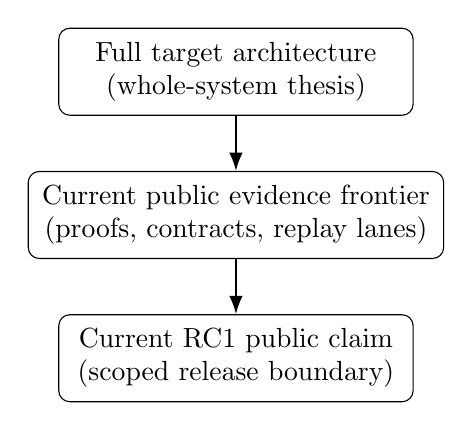
\begin{tikzpicture}[
  box/.style={draw, rounded corners, align=center, inner sep=5pt, minimum width=45mm},
  arr/.style={-Latex, thick},
  node distance=7mm
]
\node[box] (full) {Full target architecture\\(whole-system thesis)};
\node[box, below=of full] (frontier) {Current public evidence frontier\\(proofs, contracts, replay lanes)};
\node[box, below=of frontier] (rc1) {Current RC1 public claim\\(scoped release boundary)};
\draw[arr] (full) -- (frontier);
\draw[arr] (frontier) -- (rc1);
\end{tikzpicture}
\caption{Assurance boundary picture. The target architecture is broader than the current public evidence frontier, and the RC1 public claim is narrower still.}
\label{fig:boundary}
\end{figure}

\section{Guarantees and assumptions}
\begin{table}[t]
\centering
\small
\begin{tabular}{@{}L{31mm}L{23mm}L{26mm}L{54mm}@{}}
\toprule
Surface & Intended guarantee & Current strongest public evidence & Main assumptions / limits \\
\midrule
Spot winner selection & unique canonical winner on emitted bounded candidates & proved & explicit total key, nonempty admitted family, bounded emitted domain \\
Spot CPMM and fee core & reserve-bounded swap and exact accounting posture & proved & model-specific integer assumptions; dust state remains explicit \\
Settlement / quote binding & replay-verifiable canonical settlement packet & contract + proved helper shells + tests & certificate lanes must remain explicit and canonical \\
Value / price packets & meaningful value-neutral and provenance contracts & contract + tests & declared price and freshness inputs are trusted contract inputs \\
Kernel composition & inductive mirror-sync preservation & contract & cross-module facts must be synchronized, not assumed eventually consistent \\
Runtime ingress & signer / nonce / receipt consistency & contract + tests & supported HTTP boundary is narrower than the full runtime codebase \\
ZUSD / oracle safety & bounded solvency and stale-oracle fail-closed posture & mixed: proved helpers, contracts, tests & not every monetary claim is release-backed today \\
Perps / funding / liquidation & bounded risk-envelope posture & mixed: contracts, kernels, replay evidence & perps public claims remain narrower than full derivatives completeness \\
Public RC1 release & replayable clean-checkout assurance surface & contract + replay evidence & clean tree, frozen scope, green lanes, honest exclusions \\
\bottomrule
\end{tabular}
\caption{Whole-system guarantee matrix. The architecture is broad, but the public evidence class and assumption boundary vary by surface.}
\end{table}

\section{Whole-system review checklist}
For a reviewer trying to understand the full system rather than one isolated
module, the practical order is:
\begin{enumerate}
  \item review the execution and certificate planes together, because canonical
  winners only become settlement-authoritative through certificate shells;
  \item review the oracle and risk planes together, because freshness and
  provenance posture are shared preconditions for zUSD, settlement, and perps;
  \item review the runtime and control planes together, because nonce and
  ingress mistakes can invalidate otherwise correct core semantics;
  \item review the assurance plane last, because it explains which of the above
  surfaces are presently release-backed versus only architectural targets.
\end{enumerate}
Standard reading: the full system is best reviewed by dependency order rather
than by directory order.
Practical consequence: the paper is intentionally structured as a system map,
not just as a list of files.

\section{End-state proof agenda}
The finished system still needs more than the current RC1 surface. The major
remaining proof obligations are:
\begin{enumerate}
  \item widen bounded canonicality theorems into broader generator and packet
  surfaces without losing explicit candidate-domain assumptions;
  \item close more of settlement and price-provenance behavior inside kernel or
  theorem-backed packet shells;
  \item strengthen zUSD and perps from mixed contract/replay posture into
  broader proof-backed public claims;
  \item keep runtime ingress, signer, nonce, and replay surfaces aligned with
  the same canonical payload semantics proved or contracted below them;
  \item preserve the distinction between the broad architecture target and the
  narrower release-backed public claim.
\end{enumerate}

The public references that ground this paper are intentionally narrow:
\begin{itemize}
  \item \code{docs/PUBLIC_ASSURANCE_REPLAY.md}
  \item \code{docs/RC1_SCOPE.md}
  \item \code{docs/RC1_VERIFIED_SURFACE_MATRIX.md}
  \item \code{docs/TLA_CLAIM_SUMMARY.md}
  \item \code{docs/KERNEL_ABI_AND_COMPOSITION.md}
  \item \code{docs/claims_registry.yaml}
  \item theorem-bearing files under \code{lean-mathlib/Proofs/}
  \item public kernels under \code{src/kernels/dex/}
\end{itemize}

That is the core honesty rule of this whitepaper.
It describes the whole system in detail, but it only relies on public-safe
artifacts and explicitly bounded public claims.

\end{document}
